\section{Provided Test Cases}
In this section, we provide the output wave for the provided test cases. We show both full code results and the results of disabled hazard handling. Also, we show the wave of handling hazards through NOPs.

\subsection{One Operand Test Case}

\subsubsection{Full Code}
The figures \ref{fig:1op_reg_1} and \ref{fig:1op_reg_2} show the output wave of full code.
\begin{figure}[H]
    \centering
    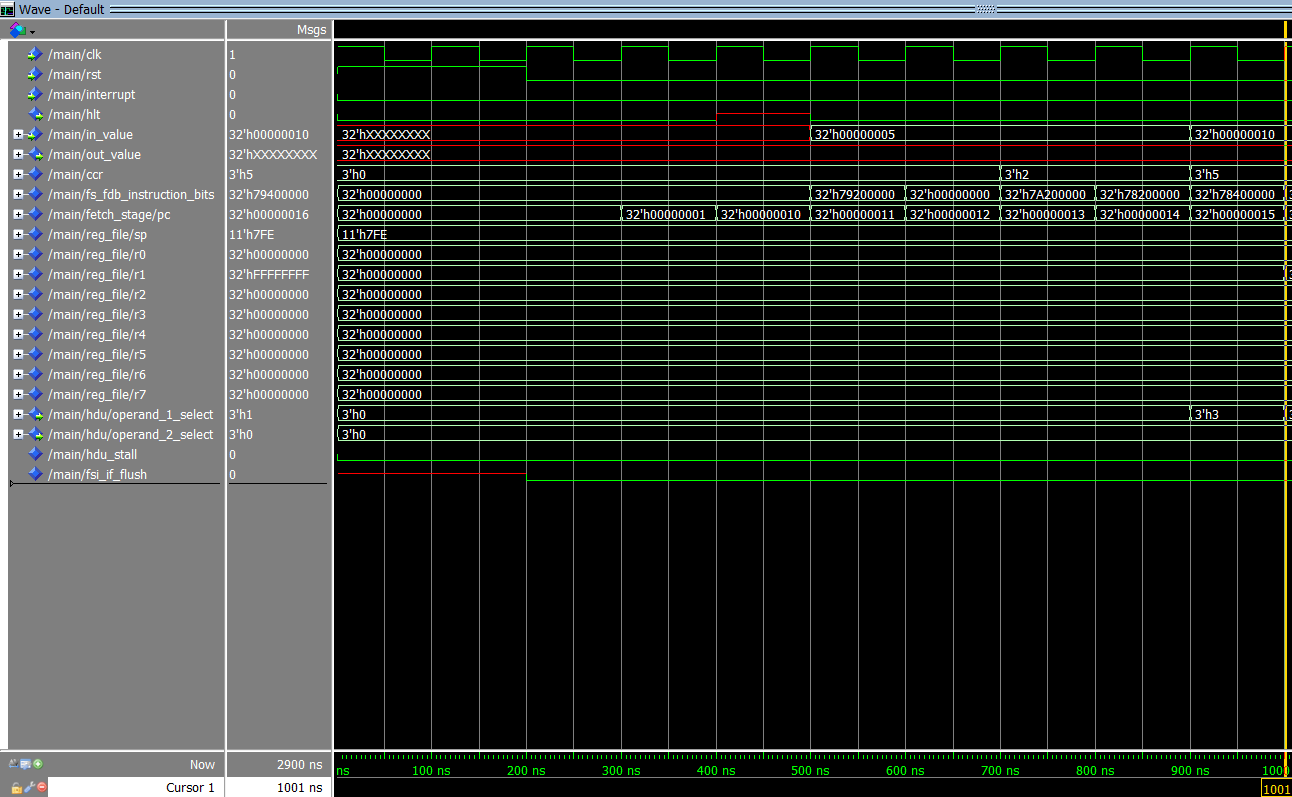
\includegraphics[width=0.9\textwidth]{images/test_cases/one_operand/OneOperand_regular_1.PNG}
    \caption{One Operand Full Code Output wave 1}
    \label{fig:1op_reg_1}
\end{figure}

\begin{figure}[H]
    \centering
    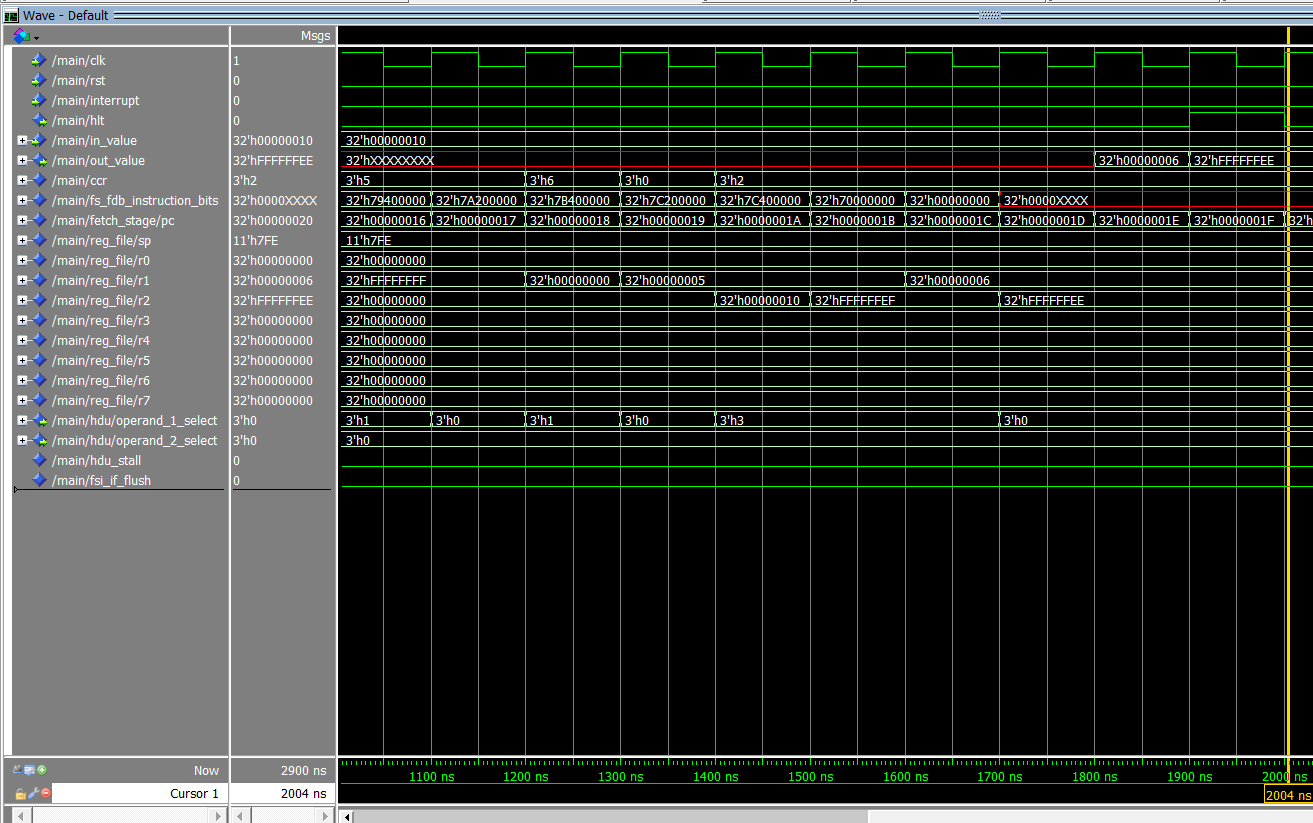
\includegraphics[width=0.9\textwidth]{images/test_cases/one_operand/OneOperand_regular_2.PNG}
    \caption{One Operand Full Code Output wave 2}
    \label{fig:1op_reg_2}
\end{figure}

\subsubsection{No Forwarding}
The figures \ref{fig:1op_no_1} and \ref{fig:1op_no_2} show the output wave of code with no forwarding.
\begin{figure}[H]
    \centering
    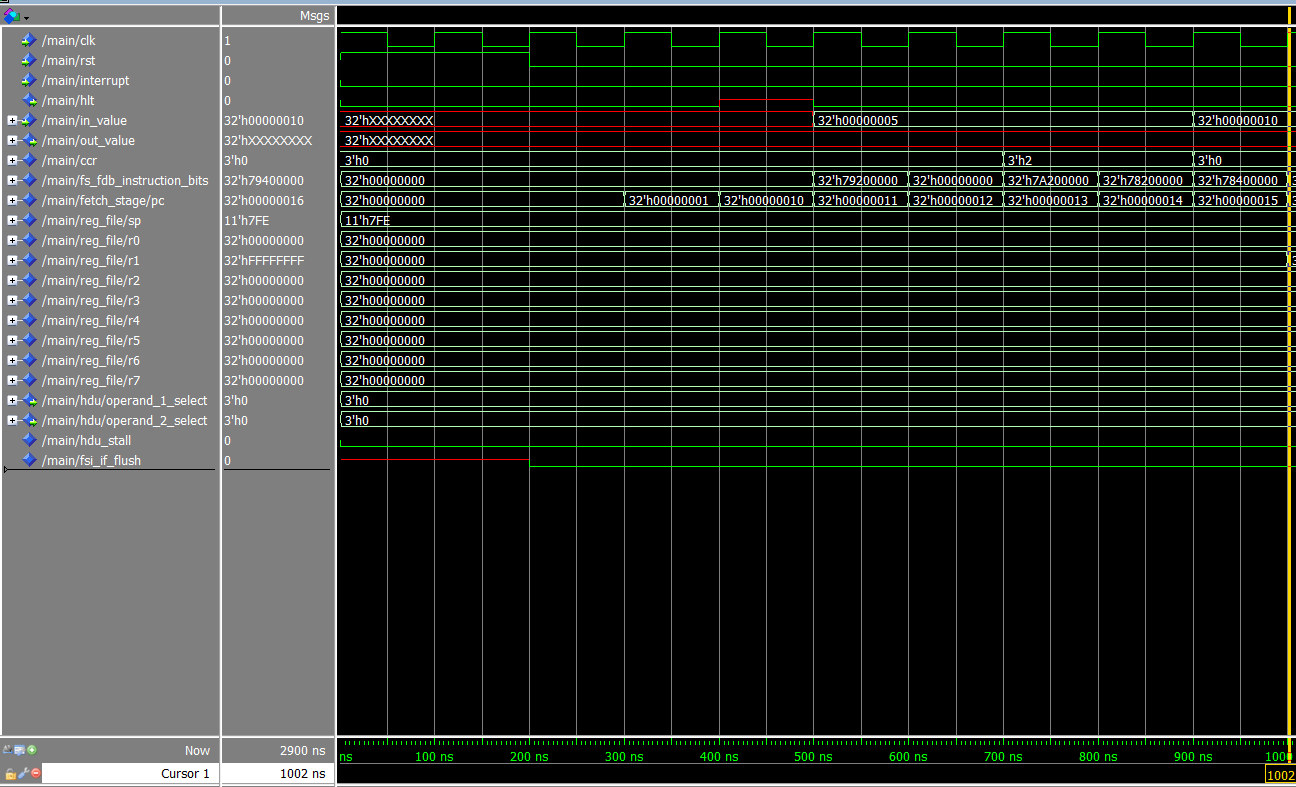
\includegraphics[width=0.9\textwidth]{images/test_cases/one_operand/OneOperand_no_forward_1.PNG}
    \caption{One Operand No Forwarding Output wave 1}
    \label{fig:1op_no_1}
\end{figure}

\begin{figure}[H]
    \centering
    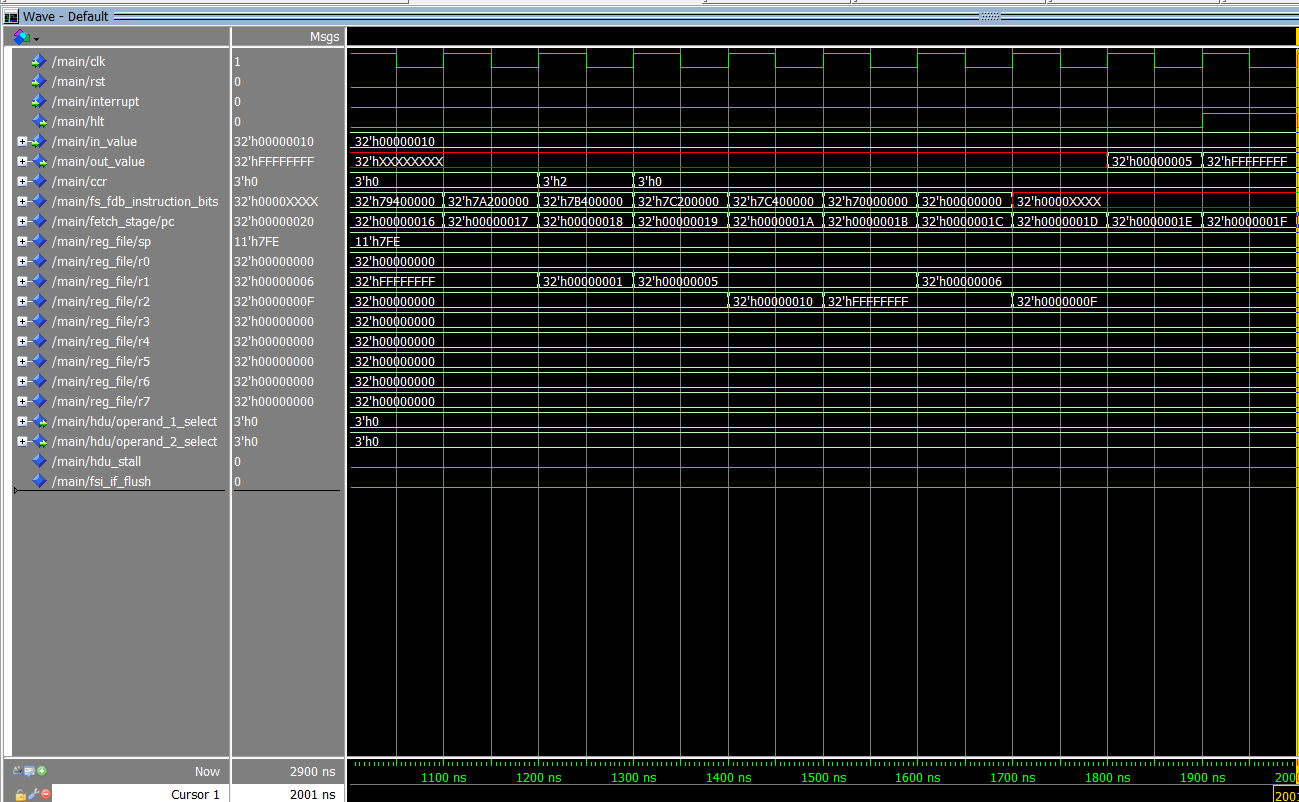
\includegraphics[width=0.9\textwidth]{images/test_cases/one_operand/OneOperand_no_forward_2.PNG}
    \caption{One Operand No Forwarding Output wave 2}
    \label{fig:1op_no_2}
\end{figure}

\subsubsection{NOPs Solution}
The figures \ref{fig:1op_nop_1}, \ref{fig:1op_nop_2} and \ref{fig:1op_nop_3} show the output wave of code with NOPs solution.
\begin{figure}[H]
    \centering
    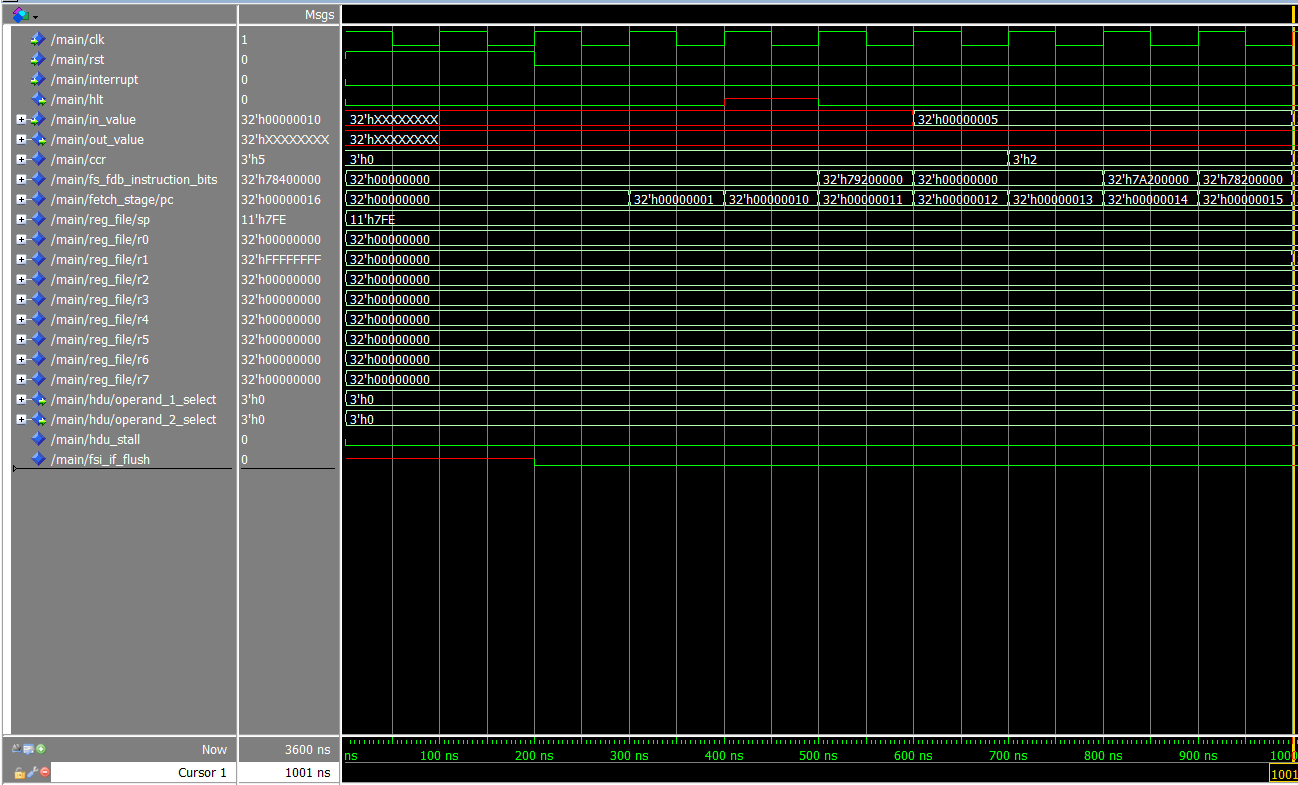
\includegraphics[width=0.9\textwidth]{images/test_cases/one_operand/OneOperand_NOP_1.PNG}
    \caption{One Operand NOPs Solution Output wave 1}
    \label{fig:1op_nop_1}
\end{figure}

\begin{figure}[H]
    \centering
    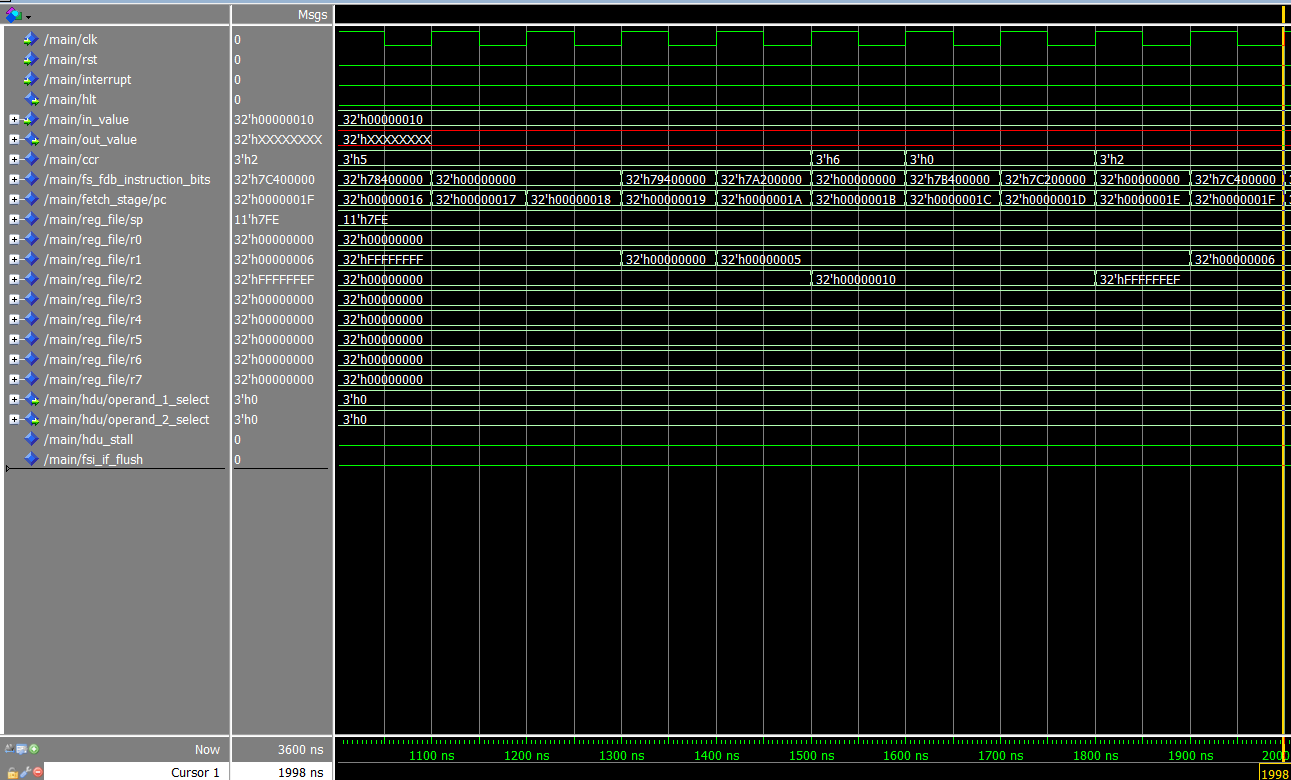
\includegraphics[width=0.9\textwidth]{images/test_cases/one_operand/OneOperand_NOP_2.PNG}
    \caption{One Operand NOPs Solution Output wave 2}
    \label{fig:1op_nop_2}
\end{figure}

\begin{figure}[H]
    \centering
    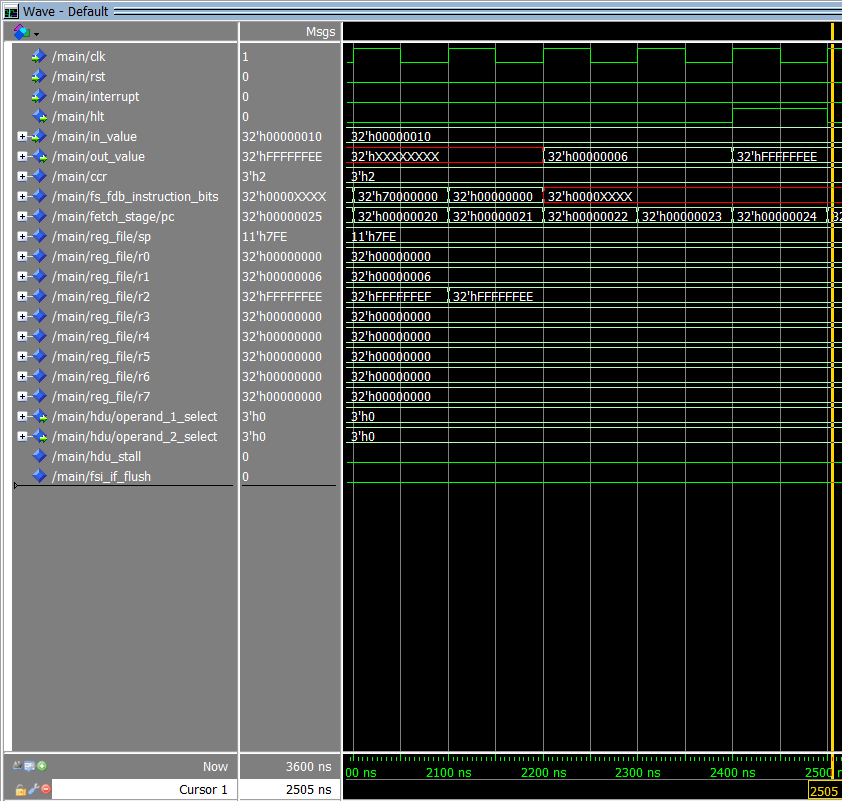
\includegraphics[width=0.9\textwidth]{images/test_cases/one_operand/OneOperand_NOP_3.PNG}
    \caption{One Operand NOPs Solution Output wave 3}
    \label{fig:1op_nop_3}
\end{figure}


\subsection{Two Operand Test Case}

\subsubsection{Full Code}
The figures \ref{fig:2op_reg_1}, \ref{fig:2op_reg_2} and \ref{fig:2op_reg_3} show the output wave of full code.
\begin{figure}[H]
    \centering
    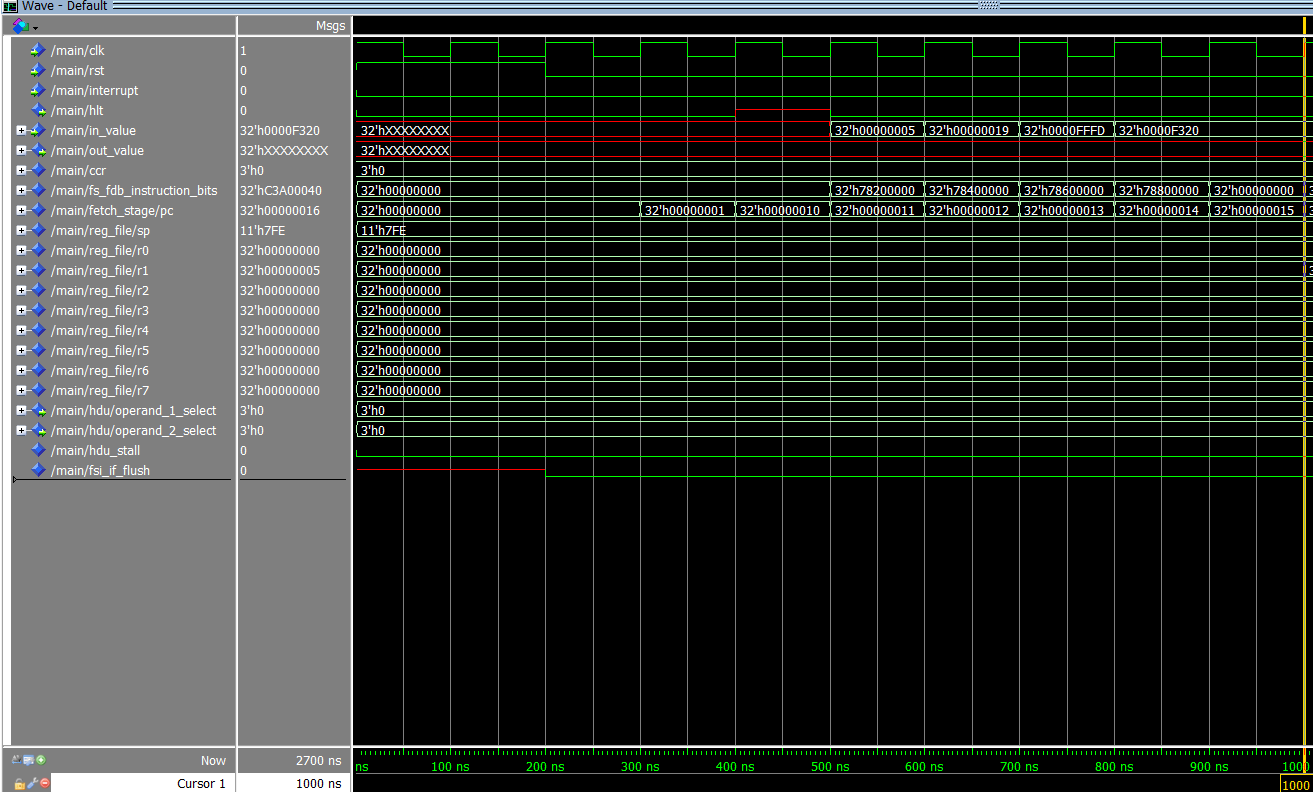
\includegraphics[width=0.9\textwidth]{images/test_cases/two_operand/TwoOperand_regular_1.PNG}
    \caption{Two Operand Full Code Output wave 1}
    \label{fig:2op_reg_1}
\end{figure}

\begin{figure}[H]
    \centering
    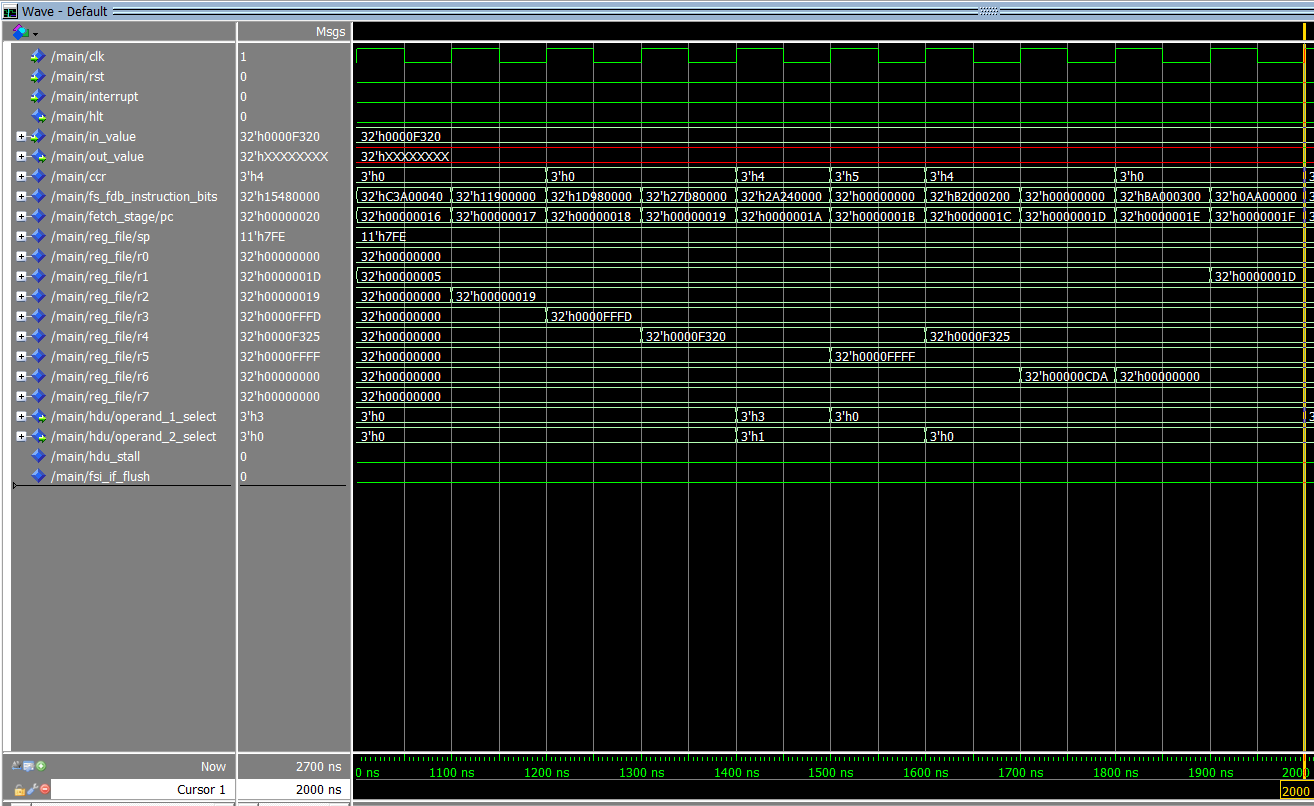
\includegraphics[width=0.9\textwidth]{images/test_cases/two_operand/TwoOperand_regular_2.PNG}
    \caption{Two Operand Full Code Output wave 2}
    \label{fig:2op_reg_2}
\end{figure}

\begin{figure}[H]
    \centering
    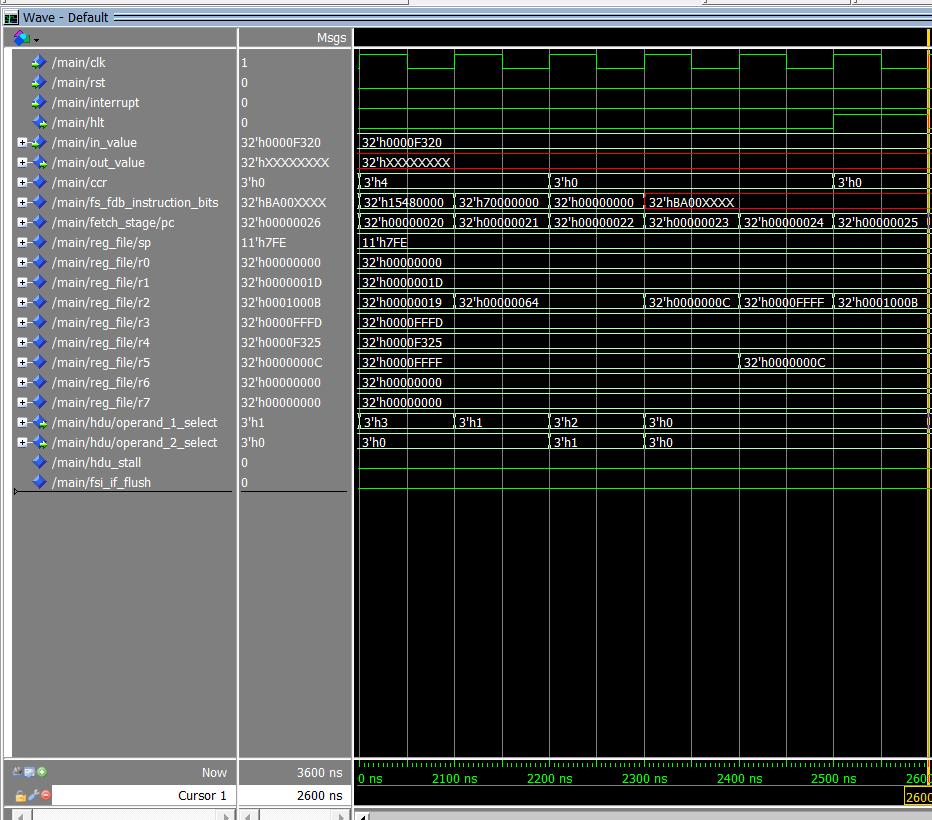
\includegraphics[width=0.9\textwidth]{images/test_cases/two_operand/TwoOperand_regular_3.PNG}
    \caption{Two Operand Full Code Output wave 3}
    \label{fig:2op_reg_3}
\end{figure}

\subsubsection{No Forwarding}
The figures \ref{fig:2op_no_1}, \ref{fig:2op_no_2} and \ref{fig:2op_no_3} show the output wave of code with no forwarding.
\begin{figure}[H]
    \centering
    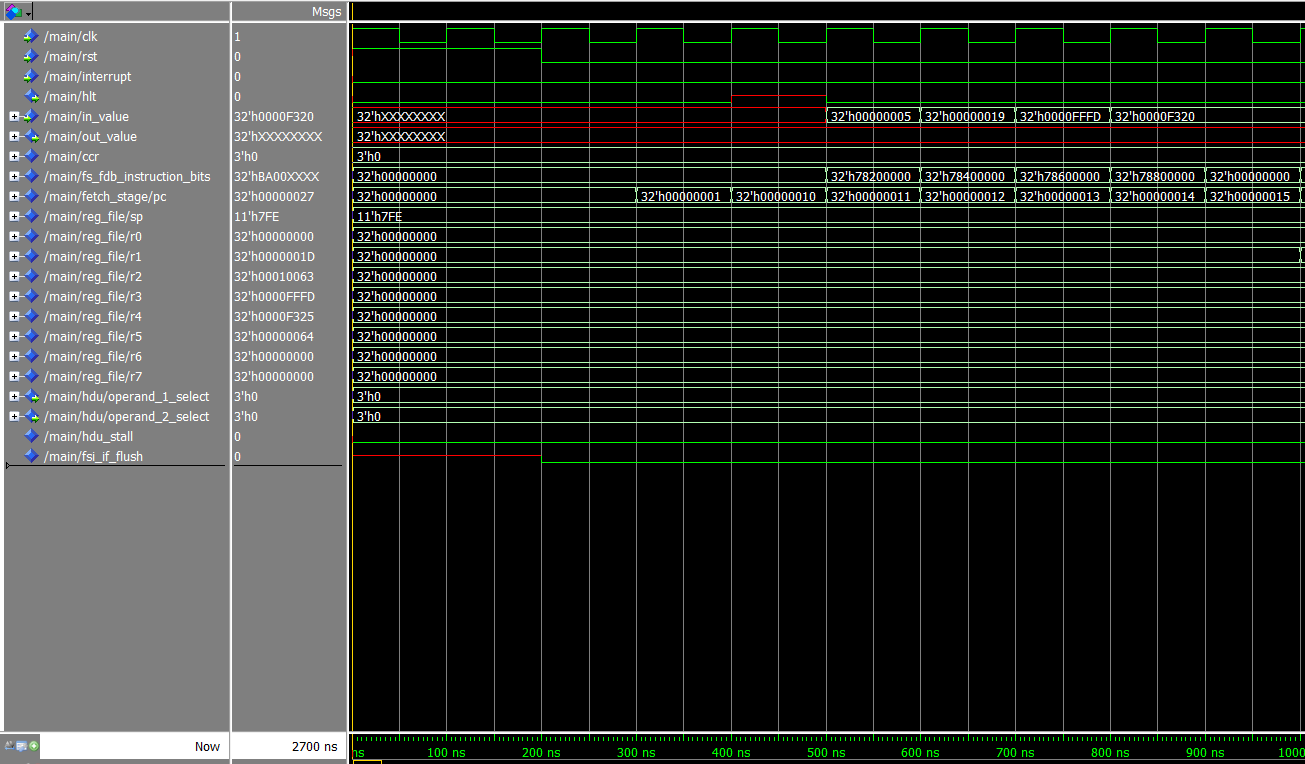
\includegraphics[width=0.9\textwidth]{images/test_cases/two_operand/TwoOperand_no_forward_1.PNG}
    \caption{Two Operand No Forwarding Output wave 1}
    \label{fig:2op_no_1}
\end{figure}

\begin{figure}[H]
    \centering
    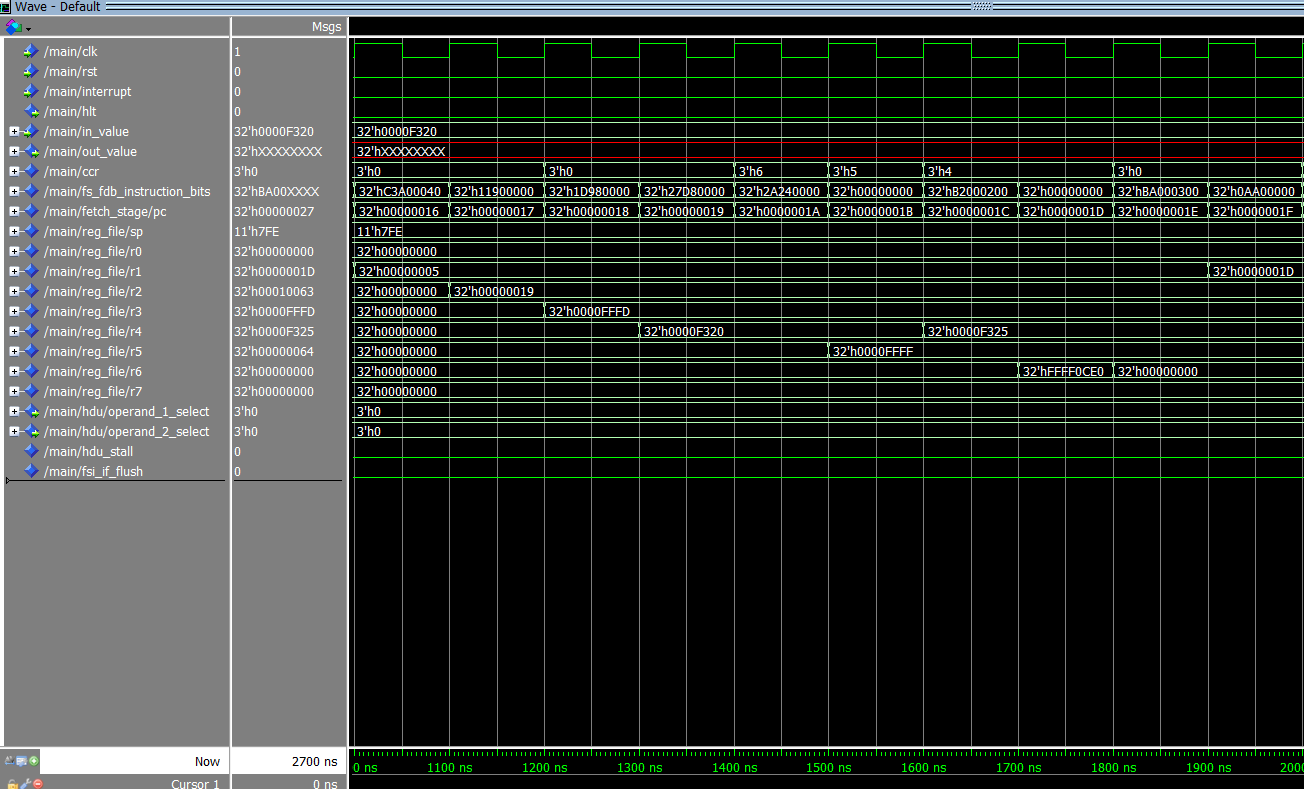
\includegraphics[width=0.9\textwidth]{images/test_cases/two_operand/TwoOperand_no_forward_2.PNG}
    \caption{Two Operand No Forwarding Output wave 2}
    \label{fig:2op_no_2}
\end{figure}

\begin{figure}[H]
    \centering
    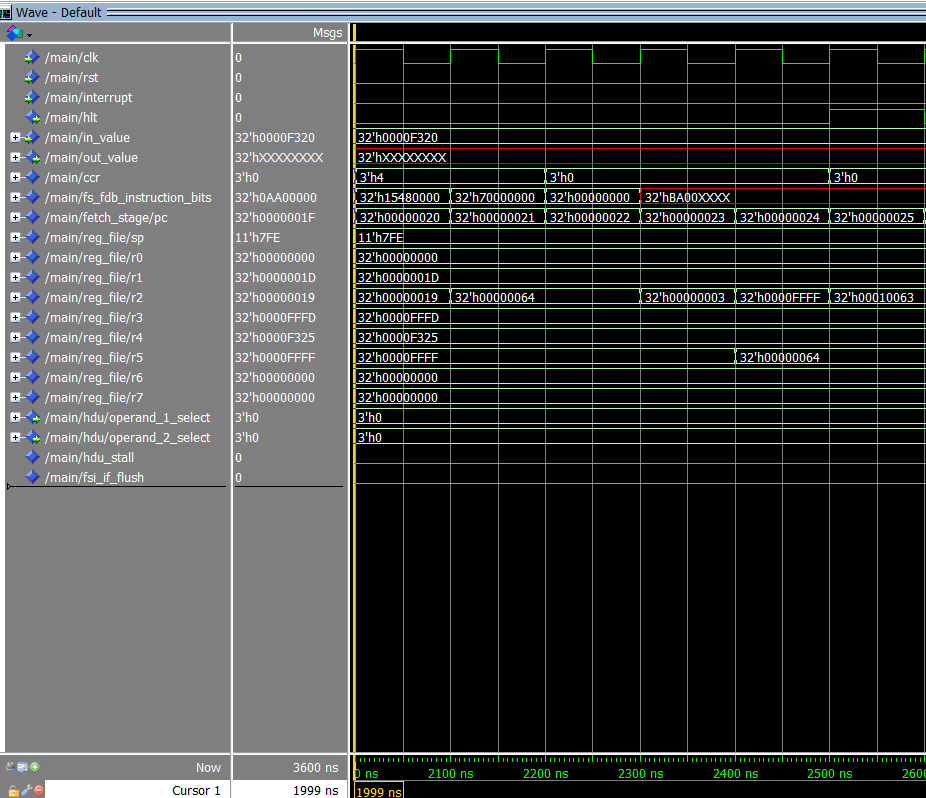
\includegraphics[width=0.9\textwidth]{images/test_cases/two_operand/TwoOperand_no_forward_3.PNG}
    \caption{Two Operand No Forwarding Output wave 3}
    \label{fig:2op_no_3}
\end{figure}

\subsubsection{NOPs Solution}
The figures \ref{fig:2op_nop_1}, \ref{fig:2op_nop_2}, \ref{fig:2op_nop_3} and \ref{fig:2op_nop_4} show the output wave of code with NOPs solution.
\begin{figure}[H]
    \centering
    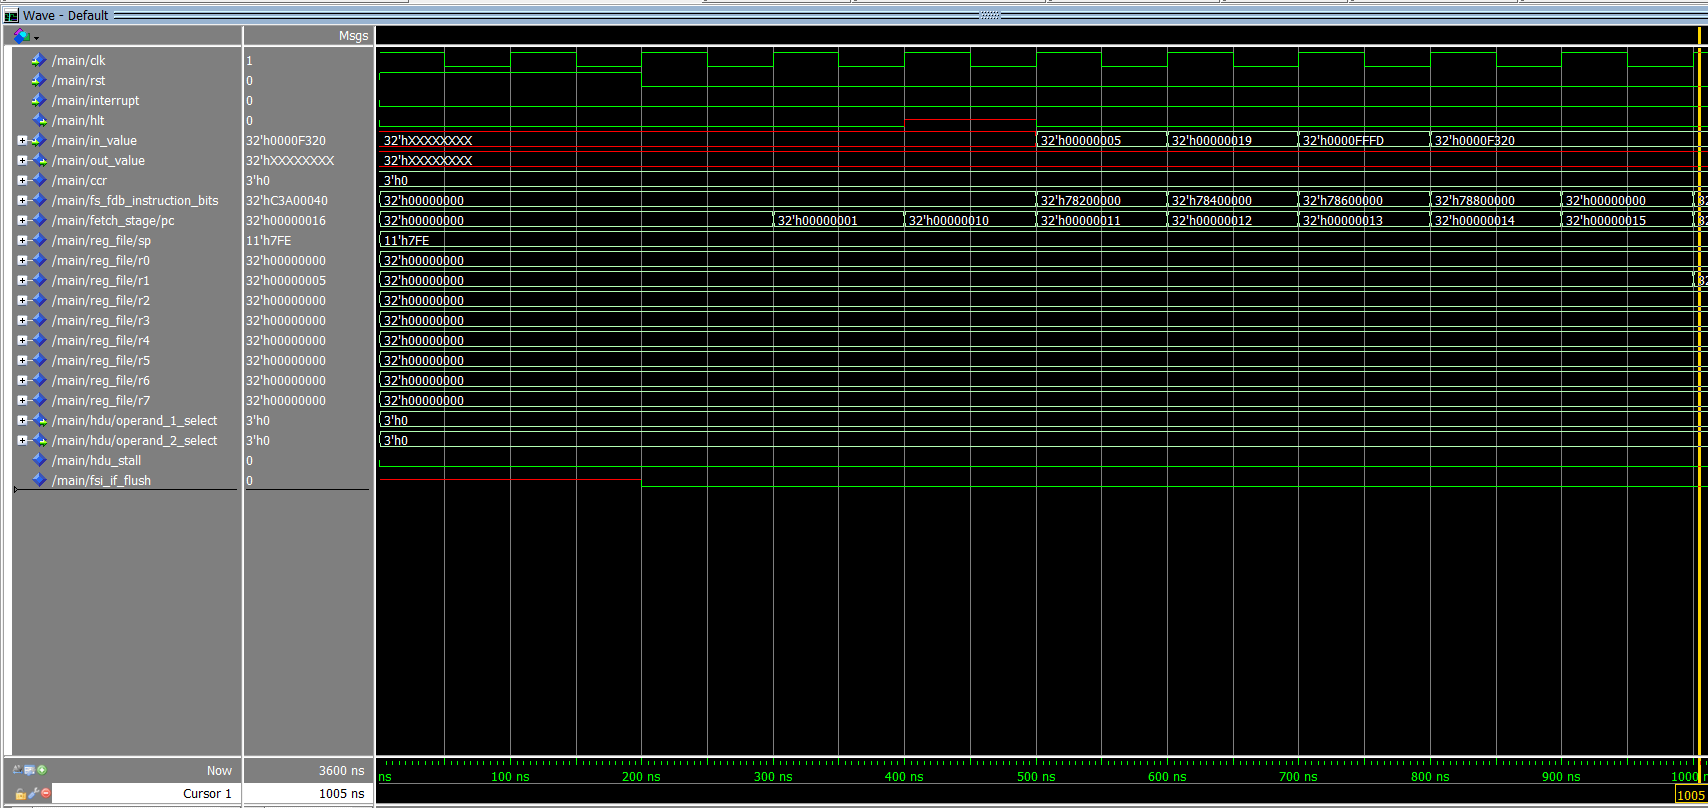
\includegraphics[width=0.9\textwidth]{images/test_cases/two_operand/TwoOperand_NOP_1.PNG}
    \caption{Two Operand NOPs Solution Output wave 1}
    \label{fig:2op_nop_1}
\end{figure}

\begin{figure}[H]
    \centering
    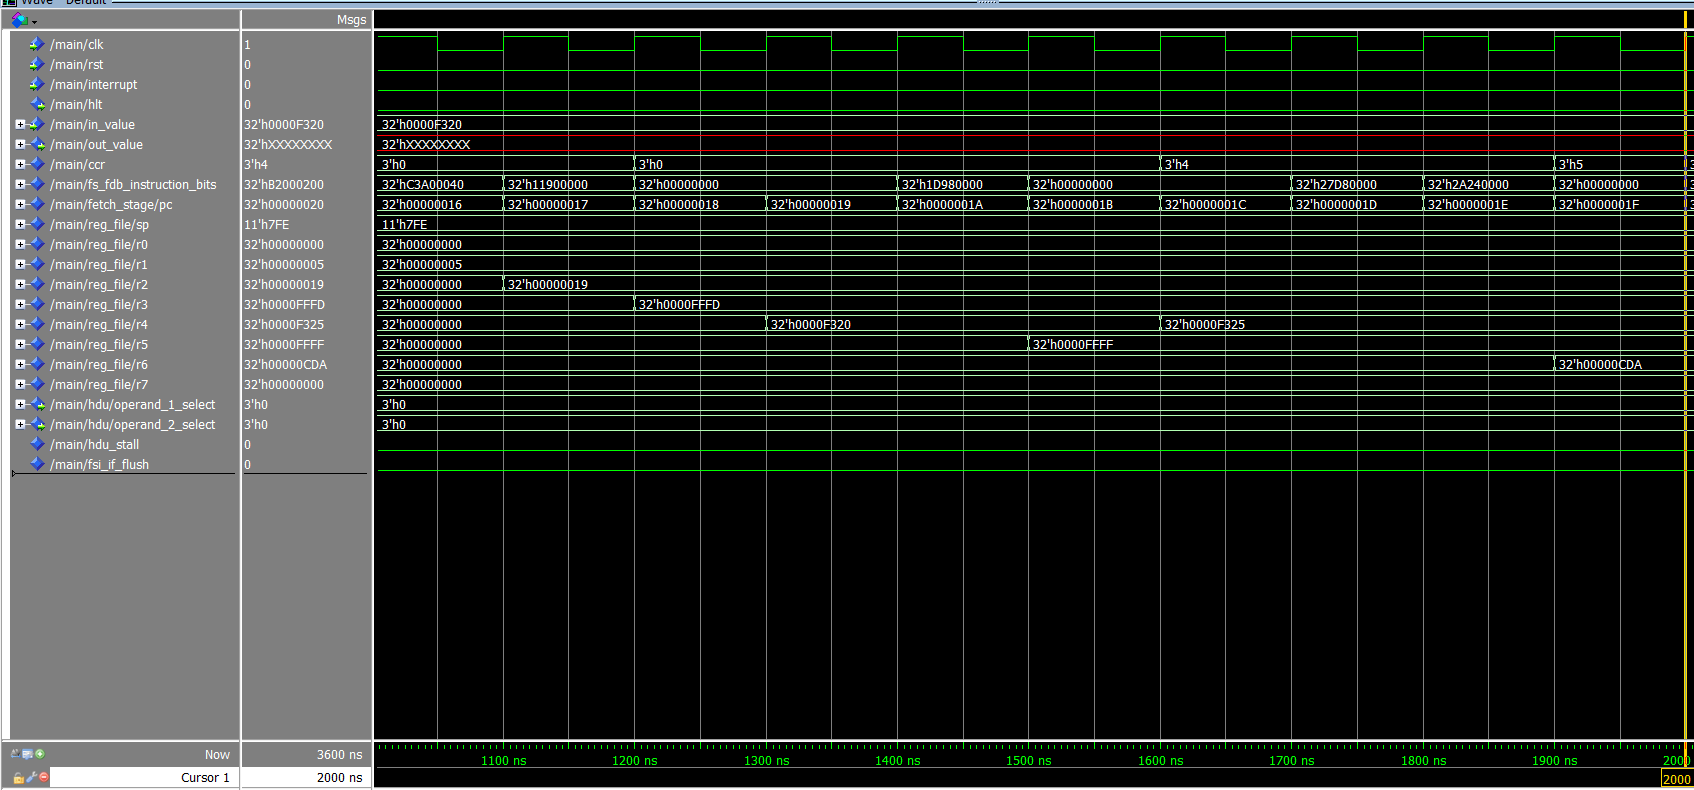
\includegraphics[width=0.9\textwidth]{images/test_cases/two_operand/TwoOperand_NOP_2.PNG}
    \caption{Two Operand NOPs Solution Output wave 2}
    \label{fig:2op_nop_2}
\end{figure}

\begin{figure}[H]
    \centering
    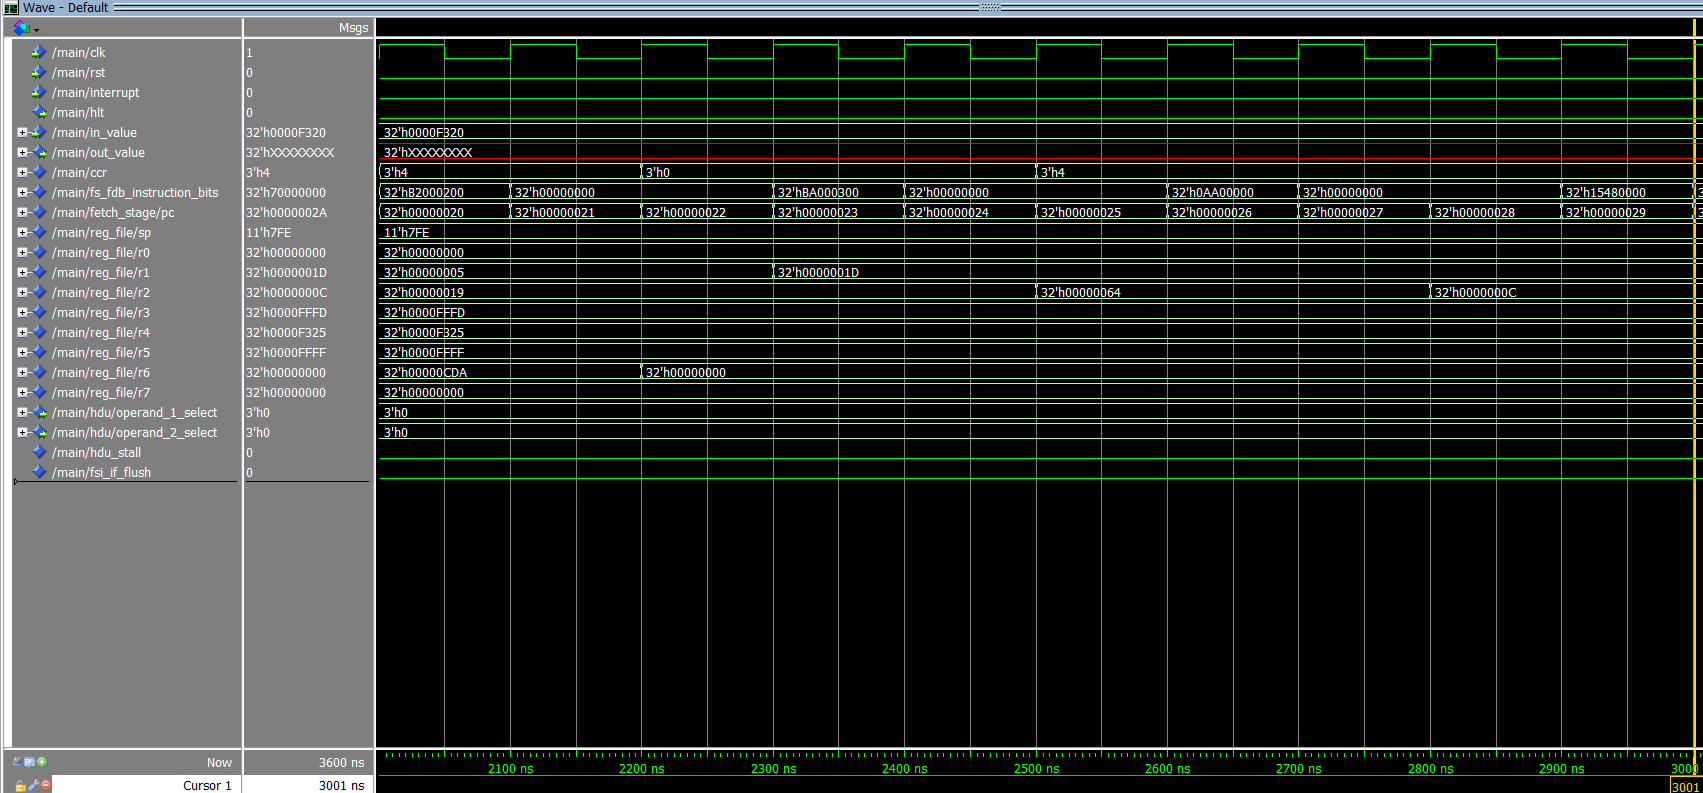
\includegraphics[width=0.9\textwidth]{images/test_cases/two_operand/TwoOperand_NOP_3.PNG}
    \caption{Two Operand NOPs Solution Output wave 3}
    \label{fig:2op_nop_3}
\end{figure}

\begin{figure}[H]
    \centering
    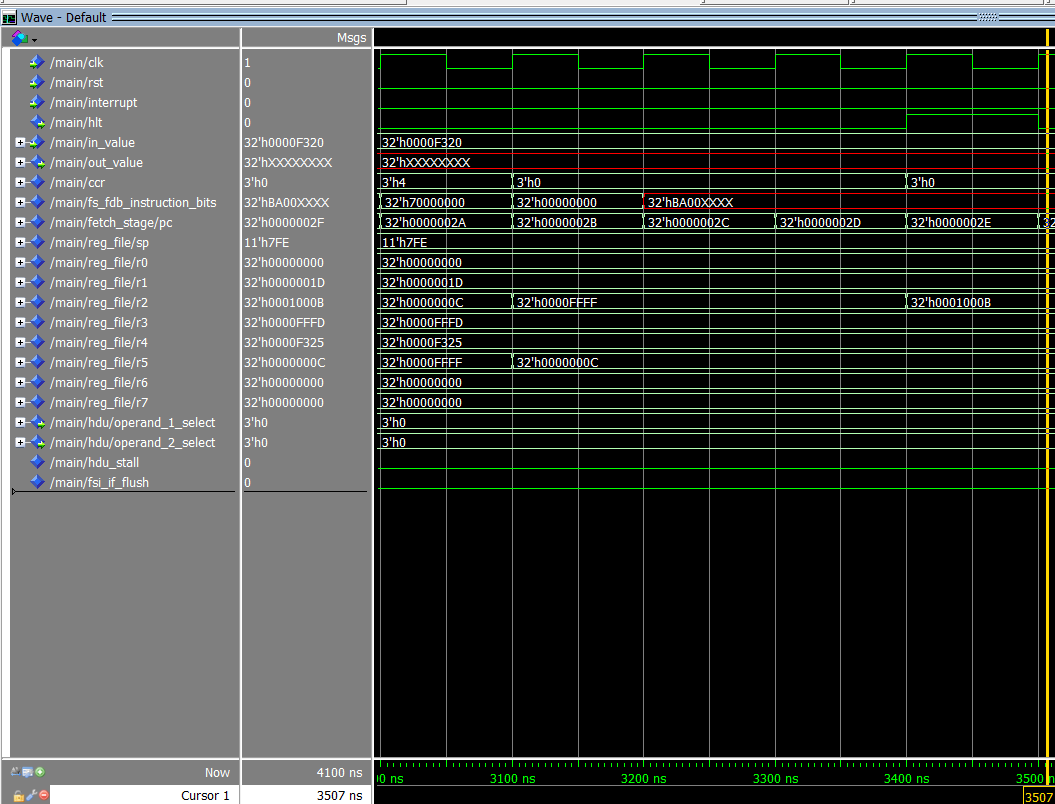
\includegraphics[width=0.9\textwidth]{images/test_cases/two_operand/TwoOperand_NOP_4.PNG}
    \caption{Two Operand NOPs Solution Output wave 4}
    \label{fig:2op_nop_4}
\end{figure}

\subsection{Memory Test Case}

\subsection{Branch Test Case}

\subsection{Branch Prediction Test Case}

\subsection{Memory Cache Test Case}
Memory cache system is not implemented. 

\section{Complete Hazard Analysis}